% ============================================================
% Cours : Séries de Fourier
% Pôle Formation UIMM - CVDL - BTS Industriel - S. JAUBERT
% Référence programme : arrêté du 4 juin 2013, module « Séries de Fourier » (p. 19-20)
% ============================================================
\documentclass[a4paper,11pt]{article}
\usepackage[utf8]{inputenc}
\usepackage[T1]{fontenc}
% babel-french absent sur certains postes : chargement conditionnel
\IfFileExists{french.ldf}{\usepackage[french]{babel}}{\renewcommand{\contentsname}{Table des matières}}
\usepackage{helvet}
\usepackage{courier}
\renewcommand{\familydefault}{\sfdefault}
\usepackage[top=3cm, bottom=2.5cm, left=2cm, right=2cm, headheight=2cm]{geometry}
\usepackage{amsmath,amssymb,amsfonts}
\usepackage{graphicx}
\usepackage[dvipsnames,table]{xcolor}
\usepackage{tikz}
\usetikzlibrary{arrows.meta, calc, positioning, mindmap, matrix}
\usepackage{pgfplots}
\pgfplotsset{compat=1.18}
\usepackage[most]{tcolorbox}
\usepackage{fancyhdr}
\usepackage{hyperref}
\usepackage{enumitem}
\usepackage{booktabs,array,multicol,needspace}

\definecolor{uimmblue}{HTML}{005C85}
\definecolor{uimmred}{HTML}{D31326}
\definecolor{uimmlightblue}{HTML}{E8F1F8}
\definecolor{uimmgray}{HTML}{333333}
\definecolor{uimmlightgray}{HTML}{F5F5F5}
\hypersetup{colorlinks=true, linkcolor=uimmblue, urlcolor=uimmblue}

\usepackage{titlesec}
\titleformat{\section}
  {\LARGE\bfseries\color{uimmblue}}{\thesection.}{0.5em}{}[\vspace{2pt}{\color{uimmblue}\titlerule[1.5pt]}]
\titleformat{\subsection}{\Large\bfseries\color{uimmblue}}{\thesubsection.}{0.5em}{}
\titleformat{\subsubsection}{\large\bfseries\color{uimmblue!80!black}}{\thesubsubsection.}{0.5em}{}
\setlist[itemize,1]{label={\color{uimmblue}\textbullet}}
\setlist[itemize,2]{label={\color{uimmblue}--}}
\setlist[enumerate,1]{label={\color{uimmblue}\textbf{\arabic*.}}}

\newtcolorbox{definition}[1][]{colback=uimmlightblue, colframe=uimmblue,
  fonttitle=\bfseries\color{white}, title={\textsf{Définition}~#1}, coltitle=white,
  boxrule=1pt, arc=3pt, left=8pt, right=8pt, top=6pt, bottom=6pt, before skip=10pt, after skip=10pt}
\newtcolorbox{theoreme}[1][]{colback=uimmlightblue!50, colframe=uimmblue!80!black,
  fonttitle=\bfseries\color{white}, title={\textsf{Théorème / Propriété}~#1}, coltitle=white,
  boxrule=1.2pt, arc=3pt, left=8pt, right=8pt, top=6pt, bottom=6pt, before skip=10pt, after skip=10pt}
\newtcolorbox{methode}[1][]{colback=green!5, colframe=green!50!black,
  fonttitle=\bfseries\color{white}, title={\textsf{Méthode}~#1}, coltitle=white,
  boxrule=1pt, arc=3pt, left=8pt, right=8pt, top=6pt, bottom=6pt, before skip=10pt, after skip=10pt}
\newtcolorbox{exemple}[1][]{colback=orange!5, colframe=orange!70!black,
  fonttitle=\bfseries\color{white}, title={\textsf{Exemple}~#1}, coltitle=white,
  boxrule=1pt, arc=3pt, left=8pt, right=8pt, top=6pt, bottom=6pt, before skip=10pt, after skip=10pt,
  breakable}
\newtcolorbox{remarque}[1][]{colback=uimmlightgray, colframe=uimmgray,
  fonttitle=\bfseries, title={\textsf{Remarque}~#1}, boxrule=0.8pt, arc=3pt,
  left=8pt, right=8pt, top=6pt, bottom=6pt, before skip=10pt, after skip=10pt}
\newtcolorbox{appliindus}[1][]{colback=uimmred!5, colframe=uimmred!80!black,
  fonttitle=\bfseries\color{white}, title={\textsf{$\triangleright$ Application industrielle}~#1}, coltitle=white,
  boxrule=1.2pt, arc=4pt, left=8pt, right=8pt, top=6pt, bottom=6pt, before skip=10pt, after skip=10pt,
  breakable}
\newtcolorbox{attention}[1][]{colback=uimmred!5, colframe=uimmred,
  fonttitle=\bfseries\color{white}, title={\textsf{Attention}~#1}, coltitle=white,
  boxrule=1pt, arc=3pt, left=8pt, right=8pt, top=6pt, bottom=6pt, before skip=10pt, after skip=10pt}
\newtcolorbox{horsprog}[1][]{colback=white, colframe=uimmgray!60, borderline={0.6pt}{2pt}{uimmgray!60, dashed},
  fonttitle=\bfseries\color{uimmgray}, colbacktitle=uimmlightgray, title={\textsf{Pour aller plus loin (hors programme)}~#1},
  boxrule=0pt, arc=3pt, left=8pt, right=8pt, top=6pt, bottom=6pt, before skip=10pt, after skip=10pt}
\newtcolorbox{calculatrice}[1][]{colback=uimmlightblue!40, colframe=uimmblue,
  fonttitle=\bfseries\color{white}, title={\textsf{Fiche calculatrice}~#1}, coltitle=white,
  boxrule=1pt, arc=3pt, left=6pt, right=6pt, top=6pt, bottom=6pt, before skip=10pt, after skip=10pt}

% Raccourcis
\newcommand{\M}[1]{\begin{pmatrix}#1\end{pmatrix}}
\newcommand{\touche}[1]{\tikz[baseline=(k.base)]\node[draw=uimmgray, fill=white, rounded corners=1.5pt,
  inner sep=1.5pt, font=\footnotesize\sffamily](k){#1};}

\pagestyle{fancy}
\fancyhf{}
\renewcommand{\headrulewidth}{0pt}
\fancyhead[L]{\raisebox{-0.5\height}{
\includegraphics[height=1.5cm]{logo_uimm_placeholder.jpg}}}
\fancyhead[C]{\begin{minipage}{8cm}\centering
  {\small\color{uimmblue}\textbf{Pôle Formation UIMM - CVDL}}\\
  {\footnotesize\color{uimmgray} BTS Industriel -- Mathématiques}\end{minipage}}
\fancyhead[R]{{\small\color{uimmblue}\textbf{MOD13}}}
\fancyfoot[C]{{\color{uimmblue}\rule{\textwidth}{1pt}}\\[2pt]
  {\footnotesize\color{uimmgray} Pôle Formation UIMM -- Centre-Val de Loire \hfill S. JAUBERT \hfill \thepage}}

\begin{document}

\begin{titlepage}
\begin{tikzpicture}[remember picture, overlay]
  \fill[uimmblue] (current page.north west) rectangle ([yshift=-4cm]current page.north east);
  \node[anchor=north west] at ([xshift=2cm, yshift=-0.5cm]current page.north west)
    {
\includegraphics[height=3cm]{logo_uimm_placeholder.jpg}};
  \node[anchor=north east, white, font=\large\bfseries] at ([xshift=-2cm, yshift=-1.5cm]current page.north east)
    {Pôle Formation UIMM - CVDL};
  \node[anchor=north east, white, font=\small, align=right] at ([xshift=-2cm, yshift=-2.2cm]current page.north east)
    {BTS Industriel -- Mathématiques\\[2pt]S. Jaubert};
  \fill[uimmred] ([yshift=-4cm]current page.north west) rectangle ([yshift=-4.4cm]current page.north east);
  \node[anchor=center, text width=14cm, align=center] at ([yshift=-0.5cm]current page.center) {
    {\fontsize{28}{34}\selectfont\bfseries\color{uimmblue} Séries de Fourier}\\[20pt]
    {\Large\color{uimmgray} Module 13}\\[12pt]
    {\large\color{uimmgray}\textit{Séries numériques, coefficients de Fourier, spectre et valeur efficace}}\\[6pt]
    {\normalsize\color{uimmgray}\textit{Les bases mathématiques de l'analyse vibratoire}}\\[24pt]
    {\color{uimmblue}$\displaystyle f(t) = a_0 + \sum_{n\geq 1}\big(a_n\cos(n\omega t) + b_n\sin(n\omega t)\big)$}
  };
  \fill[uimmblue] ([yshift=1.5cm]current page.south west) rectangle (current page.south east);
  \node[anchor=center, white, font=\small] at ([yshift=0.75cm]current page.south) {
    Pôle Formation UIMM -- Centre-Val de Loire $\bullet$ La Fabrique de l'Avenir};
\end{tikzpicture}
\end{titlepage}

\thispagestyle{fancy}
\vspace*{0.1cm}
\begin{center}
{\LARGE\bfseries\color{uimmblue} MOD13 -- Séries de Fourier}\\[6pt]
{\large\color{uimmgray} Support de cours}\\[4pt]
{\normalsize\color{uimmgray} Auteur : S. JAUBERT \hspace{1cm} Formation : BTS Industriel}
\end{center}
\vspace{0.3cm}

\begin{tcolorbox}[colback=uimmlightblue!30, colframe=uimmblue,
  title={\textbf{\textsf{Fiche du Module}}}, fonttitle=\large\bfseries\color{white},
  coltitle=white, boxrule=1.2pt, arc=4pt, left=10pt, right=10pt, top=8pt, bottom=8pt]
\renewcommand{\arraystretch}{1.3}
\begin{tabular}{@{}>{\bfseries\color{uimmblue}}l @{\hspace{12pt}} p{12cm}@{}}
Bloc / Période : & Semestre 4 \\
Module :         & {[MOD13]} Séries de Fourier \\
Thème :          & Décomposer un signal périodique en harmoniques, lire un spectre, calculer une valeur efficace : les bases mathématiques du TP d'analyse vibratoire \\
Référentiel :    & Arrêté du 4 juin 2013 (programme de mathématiques des BTS), module « Séries de Fourier ». \\
\end{tabular}
\end{tcolorbox}
\vspace{0.1cm}

\begin{tcolorbox}[colback=white, colframe=uimmblue!80!black,
  title={\textbf{\textsf{Séquences et Compétences travaillées}}}, fonttitle=\large\bfseries\color{white},
  coltitle=white, boxrule=1pt, arc=4pt, left=10pt, right=10pt, top=6pt, bottom=6pt]
\textbf{\color{uimmblue} [S01] -- Séries numériques et signaux périodiques}
\begin{itemize}[leftmargin=1.5cm, itemsep=0pt]
  \item[\textbf{\color{uimmblue}[C01]}] Reconnaître une série géométrique et connaître la condition de convergence
  \item[\textbf{\color{uimmblue}[C02]}] Connaître la condition de convergence d'une série de Riemann
  \item[\textbf{\color{uimmblue}[C03]}] Représenter graphiquement une fonction $T$-périodique continue par morceaux
  \item[\textbf{\color{uimmblue}[C04]}] Exploiter la représentation graphique d'une fonction $T$-périodique affine par morceaux (périodicité, parité, expression sur une période ou une demi-période)
\end{itemize}
\textbf{\color{uimmblue} [S02] -- Coefficients de Fourier et spectre}
\begin{itemize}[leftmargin=1.5cm, itemsep=0pt]
  \item[\textbf{\color{uimmblue}[C01]}] Calculer les coefficients de Fourier : à la main pour un créneau, au logiciel dans tous les cas
  \item[\textbf{\color{uimmblue}[C02]}] Exploiter la parité d'une fonction pour simplifier le calcul des coefficients
  \item[\textbf{\color{uimmblue}[C03]}] Représenter à l'aide d'un logiciel une somme partielle et la comparer au signal
  \item[\textbf{\color{uimmblue}[C04]}] Identifier, parmi plusieurs développements proposés, celui d'une fonction donnée
  \item[\textbf{\color{uimmblue}[C05]}] Calculer une valeur efficace exacte et approchée (formule de Parseval)
  \item[\textbf{\color{uimmblue}[C06]}] Représenter et interpréter le spectre d'amplitude d'un signal (analyse harmonique)
\end{itemize}
\end{tcolorbox}

\begin{remarque}[-- Positionnement du cours]
Prérequis : fonctions trigonométriques (MOD04), calcul intégral et intégration par parties (MOD05), suites géométriques (MOD02), nombres complexes (MOD01) pour l'encadré de la forme complexe. Ce module prépare le TP d'analyse vibratoire sur le banc ACOEM BV12.
\end{remarque}

\newpage
\tableofcontents
\newpage

% ============================================================
\needspace{7cm}
\section{Pourquoi Fourier ?}\label{sec:pourquoi}

\begin{tcolorbox}[colback=uimmlightblue!30, colframe=uimmblue, boxrule=0.8pt, arc=3pt,
  title={\textbf{\textsf{L'essentiel en une phrase}}}, fonttitle=\bfseries\color{white}, coltitle=white]
Tout signal périodique, même anguleux ou fait de chocs, est une \textbf{somme de sinusoïdes} dont les fréquences sont des \textbf{multiples entiers} de sa fréquence de répétition. Le \textbf{spectre} est la liste de ces sinusoïdes et de leurs amplitudes.
\end{tcolorbox}

\begin{appliindus}[-- Le fil rouge : le banc d'analyse vibratoire BV12]\label{ex:filrouge}
Sur le banc didactique ACOEM BV12, le moteur tourne à $1\,500$\,tr/min, soit une fréquence de rotation
\[
F_0 = \frac{1\,500}{60} = 25 \text{ Hz} \qquad\text{et une période}\qquad T = \frac{1}{F_0} = 0{,}04 \text{ s} = 40 \text{ ms.}
\]
Un accéléromètre fixé sur un palier mesure les vibrations. Le collecteur affiche le signal temporel et, surtout, son \textbf{spectre}. D'après le support de formation BV12 :
\begin{itemize}
  \item un \textbf{balourd} (masse mal répartie sur le rotor) donne une vibration quasi sinusoïdale : une seule raie à $F_0$ (raie « 1× ») ;
  \item un \textbf{désalignement} déforme le signal (deux bosses par tour) : une raie dominante à $2F_0 = 50$\,Hz (raie « 2× ») ;
  \item l'\textbf{engrènement} du pignon de $60$ dents produit $60$ chocs par tour : une raie à $60\times 25 = 1\,500$\,Hz et ses multiples.
\end{itemize}
Lire un spectre, c'est donc reconnaître des \textbf{harmoniques} : c'est exactement ce que calcule la série de Fourier.
\end{appliindus}

\begin{center}
\begin{tikzpicture}[baseline=(current bounding box.north)]
\begin{axis}[width=8.2cm, height=4.6cm, axis lines=middle, xlabel={$t/T$}, ylabel={}, xmin=0, xmax=2.1, ymin=-1.9, ymax=1.9,
  xtick={0.5,1,1.5,2}, ytick={-1,1}, samples=300, domain=0:2, legend style={font=\scriptsize, at={(0.5,-0.08)}, anchor=north, legend columns=3, draw=none},
  title style={font=\small}, title={Signal « désalignement »}]
  \addplot[uimmblue!60, dashed, thick] {sin(deg(2*pi*x))};
  \addplot[orange!80!black, dashed, thick] {0.8*sin(deg(4*pi*x))};
  \addplot[uimmred, very thick] {sin(deg(2*pi*x)) + 0.8*sin(deg(4*pi*x))};
  \legend{$\sin(\omega t)$, $0{,}8\sin(2\omega t)$, somme}
\end{axis}
\end{tikzpicture}
\hfill
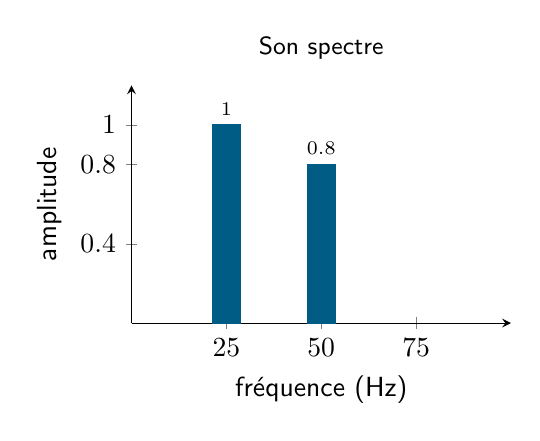
\begin{tikzpicture}[baseline=(current bounding box.north)]
\begin{axis}[width=6.4cm, height=4.6cm, ybar, bar width=10pt, xlabel={fréquence (Hz)}, ylabel={amplitude},
  ymin=0, ymax=1.2, xmin=0, xmax=100, xtick={25,50,75}, ytick={0.4,0.8,1}, axis lines=left,
  title style={font=\small}, title={Son spectre}, nodes near coords, every node near coord/.append style={font=\scriptsize}]
  \addplot[fill=uimmblue, draw=uimmblue] coordinates {(25,1) (50,0.8)};
\end{axis}
\end{tikzpicture}\\[2pt]
{\small\color{uimmgray} Un signal « à deux bosses par tour » (fondamental + harmonique 2) et son spectre : deux raies, à $25$\,Hz et $50$\,Hz.}
\end{center}

\begin{remarque}[-- Un peu d'histoire]
Joseph Fourier (1768-1830) introduit ces séries dans sa \textit{Théorie analytique de la chaleur} (1822) pour résoudre l'équation de la chaleur. Deux siècles plus tard, chaque analyseur de vibrations, chaque oscilloscope numérique et chaque codec audio en utilise une version discrète : la FFT (transformée de Fourier rapide).
\end{remarque}

% ============================================================
\needspace{7cm}
\section{Séries numériques \hfill {\normalsize\color{uimmred}[S01] [C01] [C02]}}\label{sec:series}

Un signal de Fourier est une somme d'une \textbf{infinité} de sinusoïdes. Avant de manipuler de telles sommes, il faut savoir ce que « sommer une infinité de nombres » veut dire.

\subsection{Somme partielle et convergence}\label{subsec:convergence}

\begin{definition}[-- Série numérique]
Soit $(u_n)$ une suite de nombres réels. La \textbf{somme partielle} de rang $N$ est
\[
S_N = u_0 + u_1 + \cdots + u_N = \sum_{n=0}^{N} u_n.
\]
On dit que la \textbf{série} $\sum u_n$ \textbf{converge} si $S_N$ a une limite finie $S$ quand $N\to+\infty$. On note alors $S = \displaystyle\sum_{n=0}^{+\infty} u_n$ : c'est la \textbf{somme} de la série. Sinon, la série \textbf{diverge}.
\end{definition}

\begin{tcolorbox}[colback=white, colframe=uimmblue, boxrule=0.8pt, arc=3pt]
\textbf{Analogie :} on remplit un réservoir en versant successivement $u_0$, $u_1$, $u_2$\dots\ litres. $S_N$ est le niveau après $N+1$ versements. La série converge si le niveau se stabilise ; elle diverge s'il déborde (ou oscille sans se fixer).
\end{tcolorbox}

\subsection{Séries géométriques}\label{subsec:geometriques}

\begin{theoreme}[-- Série géométrique]\label{th:geometrique}
Soit $q$ un réel. La série géométrique $\displaystyle\sum_{n\geq 0} q^n = 1 + q + q^2 + \cdots$
\begin{itemize}
  \item \textbf{converge} si et seulement si $|q| < 1$, et alors $\displaystyle\sum_{n=0}^{+\infty} q^n = \frac{1}{1-q}$ ;
  \item \textbf{diverge} si $|q|\geq 1$.
\end{itemize}
Plus généralement, pour $|q|<1$ : $\displaystyle\sum_{n=0}^{+\infty} u_0\,q^n = \frac{u_0}{1-q}$ \quad(premier terme divisé par $1 - $ raison).
\end{theoreme}

\begin{remarque}[-- D'où vient la formule ?]
La somme des termes d'une suite géométrique (MOD02) donne $S_N = \dfrac{1-q^{N+1}}{1-q}$ pour $q\neq 1$. Si $|q|<1$, $q^{N+1}\to 0$ et $S_N\to\dfrac{1}{1-q}$. Si $|q|\geq 1$, $q^{N+1}$ ne tend pas vers $0$ et $S_N$ n'a pas de limite finie.
\end{remarque}

\begin{exemple}[-- Le chemin de Zénon]\label{ex:zenon}
$1 + \frac12 + \frac14 + \frac18 + \cdots = \dfrac{1}{1-\frac12} = 2$. Une infinité de termes peut avoir une somme finie.
\end{exemple}

\begin{appliindus}[-- Graissage automatique d'un palier]\label{ex:graisse}
Un graisseur automatique injecte une dose de $d = 2$\,g de graisse dans un palier à chaque cycle. Entre deux cycles, $20\,\%$ de la graisse présente est expulsée. Juste après le $(N+1)$\textsuperscript{e} cycle, la quantité présente est (la dose injectée il y a $k$ cycles a été multipliée $k$ fois par $0{,}8$) :
\[
Q_N = 2 + 2\times 0{,}8 + 2\times 0{,}8^2 + \cdots + 2\times 0{,}8^{N} = \sum_{k=0}^{N} 2\times 0{,}8^{k}.
\]
C'est une série géométrique de premier terme $2$ et de raison $q = 0{,}8$, avec $|q|<1$ : elle converge et
\[
Q = \sum_{k=0}^{+\infty} 2\times 0{,}8^{k} = \frac{2}{1-0{,}8} = 10 \text{ g.}
\]
La quantité de graisse dans le palier se stabilise à $10$\,g, soit $5$ doses. Le technicien dimensionne le palier et le réglage du graisseur sur ce régime établi.
\end{appliindus}

\subsection{Séries de Riemann}\label{subsec:riemann}

\begin{theoreme}[-- Série de Riemann (admis)]\label{th:riemann}
Soit $\alpha$ un réel. La série $\displaystyle\sum_{n\geq 1}\frac{1}{n^{\alpha}}$ \textbf{converge si et seulement si $\alpha > 1$}.
\end{theoreme}

\begin{exemple}[-- Conjecturer au tableur]\label{ex:riemann}
Les sommes partielles $S_N = \sum_{n=1}^{N}\frac{1}{n^{\alpha}}$ calculées au tableur donnent :
\begin{center}
\renewcommand{\arraystretch}{1.3}
\begin{tabular}{|c|c|c|c|c|l|}
\hline
\rowcolor{uimmlightblue}
$N$ & $10$ & $100$ & $1\,000$ & $10\,000$ & Conjecture \\
\hline
$\alpha = \frac12$ & $5{,}02$ & $18{,}59$ & $61{,}80$ & $198{,}54$ & diverge \\
\hline
$\alpha = 1$ & $2{,}93$ & $5{,}19$ & $7{,}49$ & $9{,}79$ & diverge (lentement) \\
\hline
$\alpha = 2$ & $1{,}550$ & $1{,}635$ & $1{,}644$ & $1{,}645$ & converge ($\approx 1{,}645$) \\
\hline
$\alpha = 3$ & $1{,}198$ & $1{,}202$ & $1{,}202$ & $1{,}202$ & converge ($\approx 1{,}202$) \\
\hline
\end{tabular}
\end{center}
Pour $\alpha = 1$ (série harmonique), la somme croît sans limite, mais si lentement qu'un tableau de valeurs peut tromper : on gagne environ $2{,}3$ à chaque fois que $N$ est multiplié par $10$. Pour $\alpha = 2$, on montrera au paragraphe~\ref{sec:parseval} que la somme vaut exactement $\frac{\pi^2}{6}\approx 1{,}645$.
\end{exemple}

\begin{attention}[-- Des termes qui tendent vers 0 ne suffisent pas]
Pour $\alpha = 1$, les termes $\frac1n$ tendent vers $0$ et pourtant la série diverge. Pour qu'une série converge, il faut que ses termes tendent vers $0$, mais ce n'est pas suffisant.
\end{attention}

\begin{remarque}[-- Le lien avec les signaux]
On verra que les amplitudes des harmoniques d'un signal décroissent comme $\frac1n$ (signal avec des sauts) ou comme $\frac1{n^2}$ (signal continu avec des angles). L'énergie d'un signal fait intervenir les carrés des amplitudes, en $\frac{1}{n^2}$ ou $\frac{1}{n^4}$ : les séries de Riemann garantissent que cette énergie est finie.
\end{remarque}

% ============================================================
\needspace{7cm}
\section{Signaux périodiques \hfill {\normalsize\color{uimmred}[S01] [C03] [C04]}}\label{sec:signaux}

\subsection{Vocabulaire}\label{subsec:vocabulaire}

\begin{definition}[-- Fonction périodique]
Une fonction $f$ définie sur $\mathbb{R}$ est \textbf{périodique de période $T$} ($T>0$) si, pour tout réel $t$, $f(t+T) = f(t)$. On lui associe :
\[
\text{la fréquence } f_0 = \frac{1}{T} \ \text{(en Hz)} \qquad\text{et la pulsation } \omega = \frac{2\pi}{T} = 2\pi f_0 \ \text{(en rad/s).}
\]
$f$ est \textbf{continue par morceaux} si, sur une période, elle est continue sauf en un nombre fini de points où elle présente un saut (limites à gauche et à droite finies).
\end{definition}

\begin{methode}[-- Représenter un signal périodique]\label{meth:representer}
On trace la courbe sur une période, puis on la \textbf{recopie par translation} de $T$, $2T$, $-T$\dots\ On représente au moins deux ou trois périodes. Aux points de saut, on trace des pointillés verticaux (la valeur exacte en ce point n'a pas d'importance pour la série de Fourier).
\end{methode}

\begin{appliindus}[-- Trois signaux de l'atelier]\label{ex:troissignaux}
\textbf{Créneau d'onduleur} (tension $\pm E$) : un onduleur de moteur délivre $+E$ pendant une demi-période et $-E$ pendant l'autre.\\
\textbf{Dent de scie} (rampe) : la porteuse d'une commande MLI ou le balayage d'un capteur laser monte linéairement puis retombe brutalement.\\
\textbf{Triangle} : la porteuse triangulaire d'une MLI monte et descend linéairement.
\begin{center}
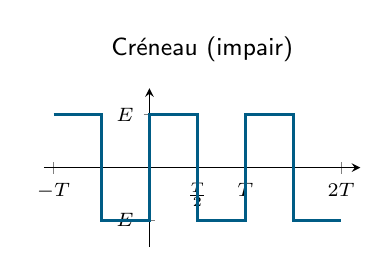
\begin{tikzpicture}
\begin{axis}[width=5.6cm, height=3.6cm, axis lines=middle, xmin=-1.1, xmax=2.2, ymin=-1.5, ymax=1.5,
  xtick={-1,-0.5,0.5,1,1.5,2}, xticklabels={$-T$,,$\frac T2$,$T$,,$2T$}, ytick={-1,1}, yticklabels={$-E$,$E$},
  title={Créneau (impair)}, title style={font=\small}, tick label style={font=\scriptsize}]
  \addplot[uimmblue, very thick, const plot] coordinates {(-1,1)(-0.5,-1)(0,1)(0.5,-1)(1,1)(1.5,-1)(2,-1)};
\end{axis}
\end{tikzpicture}
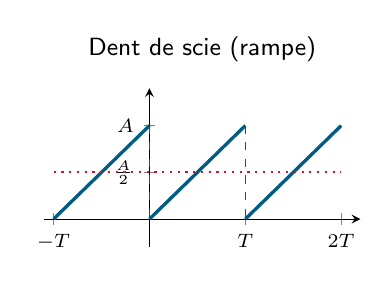
\begin{tikzpicture}
\begin{axis}[width=5.6cm, height=3.6cm, axis lines=middle, xmin=-1.1, xmax=2.2, ymin=-0.3, ymax=1.4,
  xtick={-1,1,2}, xticklabels={$-T$,$T$,$2T$}, ytick={0.5,1}, yticklabels={$\frac A2$,$A$},
  title={Dent de scie (rampe)}, title style={font=\small}, tick label style={font=\scriptsize}]
  \addplot[uimmblue, very thick] coordinates {(-1,0)(0,1)};
  \addplot[uimmblue, very thick] coordinates {(0,0)(1,1)};
  \addplot[uimmblue, very thick] coordinates {(1,0)(2,1)};
  \addplot[uimmblue, dashed] coordinates {(0,1)(0,0)};
  \addplot[uimmblue, dashed] coordinates {(1,1)(1,0)};
  \addplot[uimmred, dotted, thick] coordinates {(-1,0.5)(2,0.5)};
\end{axis}
\end{tikzpicture}
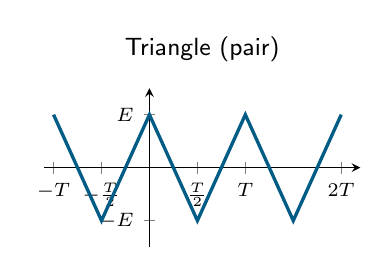
\begin{tikzpicture}
\begin{axis}[width=5.6cm, height=3.6cm, axis lines=middle, xmin=-1.1, xmax=2.2, ymin=-1.5, ymax=1.5,
  xtick={-1,-0.5,0.5,1,2}, xticklabels={$-T$,$-\frac T2$,$\frac T2$,$T$,$2T$}, ytick={-1,1}, yticklabels={$-E$,$E$},
  title={Triangle (pair)}, title style={font=\small}, tick label style={font=\scriptsize}]
  \addplot[uimmblue, very thick] coordinates {(-1,1)(-0.5,-1)(0,1)(0.5,-1)(1,1)(1.5,-1)(2,1)};
\end{axis}
\end{tikzpicture}
\end{center}
Sur la dent de scie, la droite en pointillés rouges est la \textbf{valeur moyenne} $\frac A2$.
\end{appliindus}

\subsection{Parité}\label{subsec:parite}

\begin{definition}[-- Fonction paire, fonction impaire]
\begin{itemize}
  \item $f$ est \textbf{paire} si $f(-t) = f(t)$ pour tout $t$ : la courbe est \textbf{symétrique par rapport à l'axe des ordonnées}. Exemples : $\cos$, le triangle ci-dessus.
  \item $f$ est \textbf{impaire} si $f(-t) = -f(t)$ pour tout $t$ : la courbe est \textbf{symétrique par rapport à l'origine}. Exemples : $\sin$, le créneau ci-dessus.
\end{itemize}
Un signal peut n'être ni pair ni impair : c'est le cas de la dent de scie ci-dessus.
\end{definition}

\begin{theoreme}[-- Produits et intégrales]\label{th:parite}
\begin{itemize}
  \item Règle des signes : pair $\times$ pair = pair ; impair $\times$ impair = pair ; pair $\times$ impair = impair.
  \item Si $f$ est $T$-périodique, l'intégrale sur une période ne dépend pas du point de départ :
  $\displaystyle\int_a^{a+T} f(t)\,\mathrm dt = \int_0^T f(t)\,\mathrm dt = \int_{-T/2}^{T/2} f(t)\,\mathrm dt$.
  \item Si $f$ est \textbf{paire} : $\displaystyle\int_{-a}^{a} f(t)\,\mathrm dt = 2\int_0^a f(t)\,\mathrm dt$. \quad
  Si $f$ est \textbf{impaire} : $\displaystyle\int_{-a}^{a} f(t)\,\mathrm dt = 0$.
\end{itemize}
\end{theoreme}

\subsection{Expression sur une période}\label{subsec:expression}

\begin{methode}[-- Trouver l'expression d'un signal affine par morceaux]\label{meth:expression}
Sur chaque morceau, le signal est une droite $f(t) = mt + p$. On lit deux points $(t_1\,;\,y_1)$ et $(t_2\,;\,y_2)$ de ce morceau, puis $m = \dfrac{y_2-y_1}{t_2-t_1}$ et $p$ s'obtient en remplaçant un point.
\end{methode}

\begin{exemple}[-- Le triangle sur une demi-période]\label{ex:triangleexpr}
Sur $\left[0\,;\,\frac T2\right]$, le triangle passe par $(0\,;\,E)$ et $\left(\frac T2\,;\,-E\right)$ :
\[
m = \frac{-E - E}{\frac T2 - 0} = -\frac{4E}{T}
\qquad\text{donc}\qquad
f(t) = E - \frac{4E}{T}\,t = E\left(1 - \frac{4t}{T}\right) \quad\text{pour } 0\leq t\leq\frac T2.
\]
Comme $f$ est paire, cela suffit : sur $\left[-\frac T2\,;\,0\right]$, $f(t) = E\left(1 + \frac{4t}{T}\right)$, puis on prolonge par périodicité.
\end{exemple}

% ============================================================
\needspace{7cm}
\section{Série de Fourier d'un signal \hfill {\normalsize\color{uimmred}[S02] [C01] [C02]}}\label{sec:fourier}

\subsection{Harmoniques}\label{subsec:harmoniques}

\begin{definition}[-- Harmonique de rang $n$]
Soit un signal de période $T$, de fréquence $f_0 = \frac1T$ et de pulsation $\omega = \frac{2\pi}{T}$. Pour $n\geq 1$ entier, l'\textbf{harmonique de rang $n$} est une sinusoïde de la forme
\[
a_n\cos(n\omega t) + b_n\sin(n\omega t), \qquad\text{de fréquence } n f_0.
\]
L'harmonique de rang $1$ s'appelle le \textbf{fondamental}. Le terme constant $a_0$ est la \textbf{composante continue}.
\end{definition}

\begin{exemple}[-- Les harmoniques du BV12]
Avec $f_0 = F_0 = 25$\,Hz : fondamental à $25$\,Hz, harmonique 2 à $50$\,Hz, harmonique 3 à $75$\,Hz\dots\ La raie d'engrènement à $1\,500$\,Hz est l'harmonique de rang $60$ de la rotation de l'arbre moteur.
\end{exemple}

\subsection{Coefficients de Fourier}\label{subsec:coefficients}

\begin{definition}[-- Coefficients et série de Fourier]\label{def:coefficients}
Soit $f$ une fonction $T$-périodique continue par morceaux sur $\mathbb{R}$, et $\omega = \frac{2\pi}{T}$. Ses \textbf{coefficients de Fourier} sont
\[
\boxed{a_0 = \frac1T\int_0^T f(t)\,\mathrm dt}
\qquad
\boxed{a_n = \frac2T\int_0^T f(t)\cos(n\omega t)\,\mathrm dt}
\qquad
\boxed{b_n = \frac2T\int_0^T f(t)\sin(n\omega t)\,\mathrm dt}
\quad (n\geq 1).
\]
La \textbf{série de Fourier} associée à $f$ est
\[
a_0 + \sum_{n\geq 1}\big(a_n\cos(n\omega t) + b_n\sin(n\omega t)\big).
\]
On peut intégrer sur n'importe quel intervalle de longueur $T$, par exemple $\left[-\frac T2\,;\,\frac T2\right]$.
\end{definition}

\begin{tcolorbox}[colback=white, colframe=uimmblue, boxrule=0.8pt, arc=3pt]
\textbf{À retenir.} \quad $a_0$ est la \textbf{valeur moyenne} du signal sur une période (on la lit souvent sur le graphique). \quad Devant $a_n$ et $b_n$, le facteur est $\frac{2}{T}$, pas $\frac1T$.\\
\textbf{Moyen mnémotechnique :} « $a$ comme \textbf{a}ccordé au \textbf{c}osinus, $b$ au sinus » (ordre alphabétique : $a$ avant $b$, $\cos$ avant $\sin$).
\end{tcolorbox}

\begin{remarque}[-- Une autre convention]
Certains ouvrages et logiciels écrivent la série $\frac{a_0}{2} + \sum(\dots)$ avec $a_0 = \frac2T\int_0^T f$. Le terme constant est le même, seule la notation change. Ce cours suit la convention du programme : $a_0$ est directement la valeur moyenne.
\end{remarque}

\subsection{Premier cas : le signal est déjà une somme de sinusoïdes}\label{subsec:lecture}

\begin{appliindus}[-- Lire les coefficients sans calculer d'intégrale]\label{ex:lecture}
Un capteur de proximité placé face à l'arbre moteur du BV12 délivre, en volts,
\[
u(t) = 2{,}5 + 0{,}4\cos(50\pi t) + 0{,}3\sin(50\pi t) + 0{,}2\sin(100\pi t).
\]
Le plus petit terme oscillant est en $50\pi t$ : $\omega = 50\pi$\,rad/s, $f_0 = \frac{\omega}{2\pi} = 25$\,Hz, $T = 0{,}04$\,s. Par identification avec la série de Fourier :
\[
a_0 = 2{,}5 ; \quad a_1 = 0{,}4 ;\ b_1 = 0{,}3 ; \quad a_2 = 0 ;\ b_2 = 0{,}2 ; \quad a_n = b_n = 0 \text{ pour } n\geq 3.
\]
La composante continue $2{,}5$\,V est la tension de repos du capteur. Le fondamental ($25$\,Hz) traduit la rotation de l'arbre, l'harmonique 2 ($50$\,Hz) un léger désalignement.
\end{appliindus}

\subsection{Calcul des coefficients}\label{subsec:calcul}

\begin{methode}[-- Calculer les coefficients de Fourier en 6 étapes]\label{meth:coefficients}
\begin{enumerate}
  \item Lire la période $T$ et calculer $\omega = \frac{2\pi}{T}$.
  \item Étudier la \textbf{parité} pour savoir quels coefficients sont nuls (tableau p.~\pageref{th:simplification}).
  \item Écrire l'expression de $f$ sur une période (ou une demi-période) bien choisie.
  \item Calculer les intégrales, morceau par morceau, en utilisant si besoin l'intégration par parties.
  \item Simplifier avec $\boxed{\sin(n\pi) = 0}$ et $\boxed{\cos(n\pi) = (-1)^n}$ pour $n$ entier (et donc $\sin(2n\pi) = 0$, $\cos(2n\pi) = 1$).
  \item Contrôler : $a_0$ est-il bien la valeur moyenne lue sur le graphique ?
\end{enumerate}
\end{methode}

\begin{theoreme}[-- Simplifications dues à la parité]\label{th:simplification}
\begin{center}
\renewcommand{\arraystretch}{1.6}
\begin{tabular}{|l|c|c|}
\hline
\rowcolor{uimmlightblue}
 & $f$ \textbf{paire} & $f$ \textbf{impaire} \\
\hline
$a_0$ & $\dfrac2T\displaystyle\int_0^{T/2} f(t)\,\mathrm dt$ & $0$ \\
\hline
$a_n$ & $\dfrac4T\displaystyle\int_0^{T/2} f(t)\cos(n\omega t)\,\mathrm dt$ & $0$ \\
\hline
$b_n$ & $0$ & $\dfrac4T\displaystyle\int_0^{T/2} f(t)\sin(n\omega t)\,\mathrm dt$ \\
\hline
Série & que des cosinus & que des sinus \\
\hline
\end{tabular}
\end{center}
\textbf{Justification :} si $f$ est paire, $f(t)\sin(n\omega t)$ est impaire (pair $\times$ impair), donc son intégrale sur $\left[-\frac T2\,;\,\frac T2\right]$ est nulle ; $f(t)\cos(n\omega t)$ est paire, donc son intégrale vaut deux fois celle sur $\left[0\,;\,\frac T2\right]$. Même raisonnement pour $f$ impaire.
\end{theoreme}

\begin{appliindus}[-- Le créneau d'onduleur (calcul à la main)]\label{ex:creneau}
On considère le créneau impair de période $T$ : $f(t) = E$ sur $\left]0\,;\,\frac T2\right[$ et $f(t) = -E$ sur $\left]-\frac T2\,;\,0\right[$ (figure p.~\pageref{ex:troissignaux}).

\textbf{Parité.} $f$ est impaire, donc $a_0 = 0$ et $a_n = 0$ pour tout $n$.

\textbf{Calcul de $b_n$.} Sur $\left]0\,;\,\frac T2\right[$, $f(t) = E$ :
\[
b_n = \frac4T\int_0^{T/2} E\sin(n\omega t)\,\mathrm dt
= \frac{4E}{T}\left[-\frac{\cos(n\omega t)}{n\omega}\right]_0^{T/2}
= \frac{4E}{T\,n\omega}\Big(1 - \cos\big(n\omega\tfrac T2\big)\Big).
\]
Or $\omega\frac T2 = \frac{2\pi}{T}\times\frac T2 = \pi$ et $T\,n\omega = 2n\pi$. Donc
\[
b_n = \frac{2E}{n\pi}\big(1 - \cos(n\pi)\big) = \frac{2E}{n\pi}\big(1 - (-1)^n\big)
=
\begin{cases} 0 & \text{si } n \text{ est pair,}\\[4pt] \dfrac{4E}{n\pi} & \text{si } n \text{ est impair.}\end{cases}
\]
\textbf{Série de Fourier du créneau :}
\[
\boxed{f(t) = \frac{4E}{\pi}\left(\sin(\omega t) + \frac{\sin(3\omega t)}{3} + \frac{\sin(5\omega t)}{5} + \cdots\right) = \frac{4E}{\pi}\sum_{k\geq 0}\frac{\sin\big((2k+1)\omega t\big)}{2k+1}}
\]
Seuls les harmoniques \textbf{impairs} sont présents, et leurs amplitudes décroissent en $\frac1n$.
\end{appliindus}

\begin{remarque}[-- Référentiel]
Le calcul à la main du créneau figure dans le programme général du module « Séries de Fourier ». Pour les BTS ATI, cette capacité est retirée du référentiel ; elle est conservée ici parce qu'elle fait comprendre d'où viennent les harmoniques impairs.
\end{remarque}

\begin{appliindus}[-- La dent de scie (intégration par parties)]\label{ex:rampe}
La rampe de période $T$ vaut $f(t) = \frac{A}{T}\,t$ sur $[0\,;\,T[$ (figure p.~\pageref{ex:troissignaux}). Elle n'est ni paire ni impaire.

\textbf{Valeur moyenne.} $a_0 = \dfrac1T\displaystyle\int_0^T\frac AT\,t\,\mathrm dt = \frac{A}{T^2}\left[\frac{t^2}{2}\right]_0^T = \frac A2$ (aire du triangle divisée par $T$).

\textbf{Calcul de $b_n$.} Par parties, avec $u = t$, $v' = \sin(n\omega t)$, donc $u' = 1$, $v = -\frac{\cos(n\omega t)}{n\omega}$ :
\[
\int_0^T t\sin(n\omega t)\,\mathrm dt
= \left[-\frac{t\cos(n\omega t)}{n\omega}\right]_0^T + \frac{1}{n\omega}\int_0^T\cos(n\omega t)\,\mathrm dt
\]
\[
\phantom{\int_0^T t\sin(n\omega t)\,\mathrm dt}= -\frac{T\cos(2n\pi)}{n\omega} + \frac{1}{n\omega}\left[\frac{\sin(n\omega t)}{n\omega}\right]_0^T
= -\frac{T}{n\omega}.
\]
D'où $b_n = \dfrac2T\times\dfrac AT\times\left(-\dfrac{T}{n\omega}\right) = -\dfrac{2A}{n\omega T} = -\dfrac{A}{n\pi}$.

\textbf{Calcul de $a_n$.} Le même calcul avec $\cos$ donne $\int_0^T t\cos(n\omega t)\,\mathrm dt = 0$, donc $a_n = 0$.
\[
\boxed{f(t) = \frac A2 - \frac A\pi\left(\sin(\omega t) + \frac{\sin(2\omega t)}{2} + \frac{\sin(3\omega t)}{3} + \cdots\right)}
\]
Tous les harmoniques sont présents, en $\frac1n$. \textbf{Contrôle :} $f - \frac A2$ est impaire (symétrie par rapport au point $\left(0\,;\,\frac A2\right)$), ce qui explique $a_n = 0$.
\end{appliindus}

\begin{appliindus}[-- Le triangle (au logiciel)]\label{ex:triangle}
Pour le triangle pair d'amplitude $E$ (expression p.~\pageref{ex:triangleexpr}), $b_n = 0$ et $a_0 = 0$ (autant d'aire au-dessus qu'en dessous de l'axe). Le logiciel de calcul formel (fiche en annexe) donne
\[
a_n = \frac4T\int_0^{T/2}E\left(1-\frac{4t}{T}\right)\cos(n\omega t)\,\mathrm dt =
\begin{cases} 0 & \text{si } n \text{ pair,}\\[4pt] \dfrac{8E}{n^2\pi^2} & \text{si } n \text{ impair,}\end{cases}
\]
\[
f(t) = \frac{8E}{\pi^2}\left(\cos(\omega t) + \frac{\cos(3\omega t)}{9} + \frac{\cos(5\omega t)}{25} + \cdots\right).
\]
Les amplitudes décroissent en $\frac{1}{n^2}$, bien plus vite que pour le créneau : le triangle est continu, il n'a pas de saut.
\end{appliindus}

\subsection{Spectre d'amplitude}\label{subsec:spectre}

\begin{definition}[-- Amplitude d'un harmonique, spectre]\label{def:spectre}
Pour $n\geq 1$, l'\textbf{amplitude} de l'harmonique de rang $n$ est
\[
A_n = \sqrt{a_n^2 + b_n^2}\,, \qquad\text{car}\qquad a_n\cos(n\omega t) + b_n\sin(n\omega t) = A_n\cos(n\omega t - \varphi_n)
\]
pour un déphasage $\varphi_n$ convenable. Le \textbf{spectre d'amplitude} est le diagramme en bâtons des $A_n$ en fonction de la fréquence $nf_0$ (avec la composante continue $|a_0|$ à la fréquence $0$).
\end{definition}

\begin{exemple}[-- Retour au capteur de proximité]\label{ex:spectrecapteur}
Pour $u(t)$ (p.~\pageref{ex:lecture}) : $A_1 = \sqrt{0{,}4^2 + 0{,}3^2} = 0{,}5$\,V à $25$\,Hz et $A_2 = \sqrt{0^2 + 0{,}2^2} = 0{,}2$\,V à $50$\,Hz. Le fondamental combine un cosinus et un sinus : c'est une seule sinusoïde d'amplitude $0{,}5$\,V, décalée dans le temps.
\end{exemple}

\begin{center}
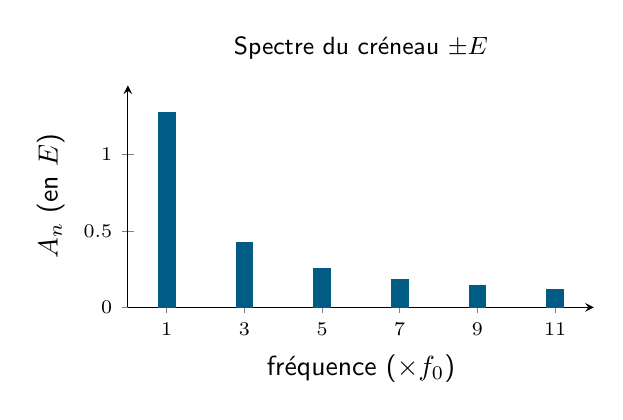
\begin{tikzpicture}
\begin{axis}[width=7.5cm, height=4.4cm, ybar, bar width=6pt, xlabel={fréquence ($\times f_0$)}, ylabel={$A_n$ (en $E$)},
  ymin=0, ymax=1.45, xmin=0, xmax=12, xtick={1,3,5,7,9,11}, axis lines=left,
  title style={font=\small}, title={Spectre du créneau $\pm E$}, tick label style={font=\scriptsize}]
  \addplot[fill=uimmblue, draw=uimmblue] coordinates {(1,1.2732)(3,0.4244)(5,0.2546)(7,0.1819)(9,0.1415)(11,0.1157)};
\end{axis}
\end{tikzpicture}
\hfill
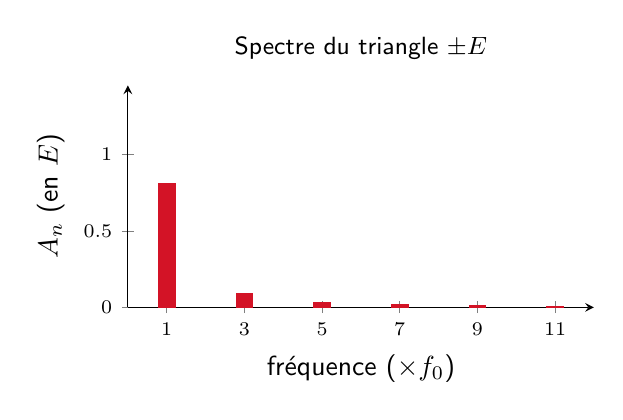
\begin{tikzpicture}
\begin{axis}[width=7.5cm, height=4.4cm, ybar, bar width=6pt, xlabel={fréquence ($\times f_0$)}, ylabel={$A_n$ (en $E$)},
  ymin=0, ymax=1.45, xmin=0, xmax=12, xtick={1,3,5,7,9,11}, axis lines=left,
  title style={font=\small}, title={Spectre du triangle $\pm E$}, tick label style={font=\scriptsize}]
  \addplot[fill=uimmred, draw=uimmred] coordinates {(1,0.8106)(3,0.0901)(5,0.0324)(7,0.0165)(9,0.0100)(11,0.0067)};
\end{axis}
\end{tikzpicture}
\end{center}
\begin{center}\small\color{uimmgray}
Deux signaux de même période et de même amplitude crête : le créneau, avec ses sauts, a des harmoniques bien plus forts que le triangle.
\end{center}

\begin{horsprog}[-- Forme complexe et « roue de Fourier »]\label{hp:complexe}
On pose, pour $n\geq 1$, $C_n = a_n - \mathrm i\,b_n$. Alors $\mathrm{Re}\big(C_n\,\mathrm e^{\mathrm i n\omega t}\big) = a_n\cos(n\omega t) + b_n\sin(n\omega t)$ et
\[
f(t) = a_0 + \mathrm{Re}\left(\sum_{n\geq 1} C_n\,\mathrm e^{\mathrm i n\omega t}\right),
\qquad
C_n = \frac2T\int_0^T f(t)\,\mathrm e^{-\mathrm i n\omega t}\,\mathrm dt,
\qquad
|C_n| = A_n.
\]
\textbf{Image mécanique :} chaque terme $C_n\,\mathrm e^{\mathrm i n\omega t}$ est un vecteur tournant de longueur $A_n$ qui fait $n$ tours par période. En mettant ces vecteurs bout à bout (une roue sur une roue\dots), l'extrémité de la chaîne dessine le signal : c'est la « roue de Fourier ». L'analyseur mesure la longueur de chaque vecteur, c'est-à-dire le spectre.\\
Autre écriture fréquente (FFT, logiciels) : $f(t) = \sum_{n\in\mathbb Z} c_n\,\mathrm e^{\mathrm i n\omega t}$ avec $c_0 = a_0$ et $c_n = \frac{C_n}{2}$ pour $n\geq 1$.
\end{horsprog}

% ============================================================
\needspace{7cm}
\section{Convergence et sommes partielles \hfill {\normalsize\color{uimmred}[S02] [C03] [C04]}}\label{sec:convergence}

\subsection{Théorème de Dirichlet}\label{subsec:dirichlet}

\begin{theoreme}[-- Conditions de Dirichlet (admis)]\label{th:dirichlet}
Soit $f$ une fonction $T$-périodique, de classe $C^1$ par morceaux sur $\mathbb{R}$ (dérivable par morceaux, avec une dérivée continue par morceaux). Alors sa série de Fourier converge en tout point $t$ :
\begin{itemize}
  \item vers $f(t)$ si $f$ est continue en $t$ ;
  \item vers la \textbf{moyenne des limites à gauche et à droite} $\dfrac{f(t^-) + f(t^+)}{2}$ si $f$ présente un saut en $t$.
\end{itemize}
Tous les signaux étudiés dans ce cours vérifient ces conditions.
\end{theoreme}

\begin{definition}[-- Somme partielle de rang $N$]
$S_N(t) = a_0 + \displaystyle\sum_{n=1}^{N}\big(a_n\cos(n\omega t) + b_n\sin(n\omega t)\big)$ : c'est le signal reconstitué avec les $N$ premiers harmoniques.
\end{definition}

\begin{center}
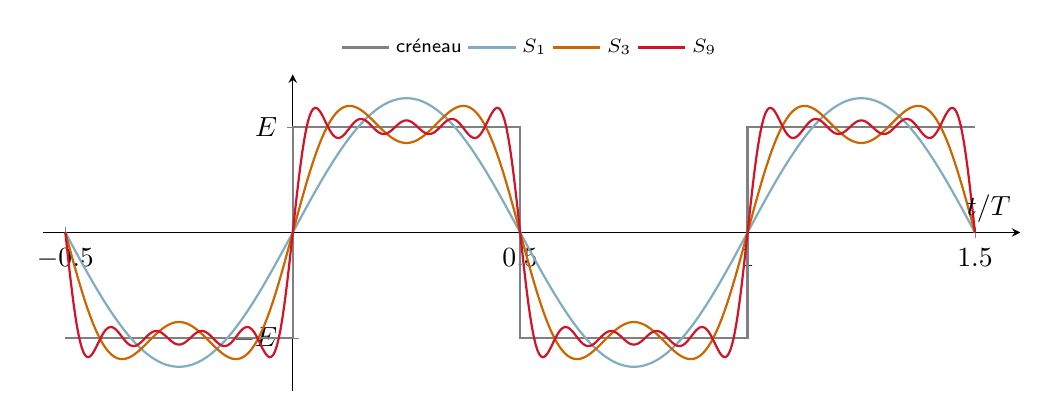
\begin{tikzpicture}
\begin{axis}[width=14cm, height=5.6cm, axis lines=middle, xlabel={$t/T$}, xmin=-0.55, xmax=1.6, ymin=-1.5, ymax=1.5,
  xtick={-0.5,0.5,1,1.5}, ytick={-1,1}, yticklabels={$-E$,$E$}, samples=500, domain=-0.5:1.5,
  legend style={font=\scriptsize, at={(0.5,1.02)}, anchor=south, legend columns=4, draw=none}]
  \addplot[black!50, thick, const plot] coordinates {(-0.5,-1)(0,1)(0.5,-1)(1,1)(1.5,1)};
  \addplot[uimmblue!50, thick] {4/pi*sin(deg(2*pi*x))};
  \addplot[orange!80!black, thick] {4/pi*(sin(deg(2*pi*x)) + sin(deg(6*pi*x))/3)};
  \addplot[uimmred, thick] {4/pi*(sin(deg(2*pi*x)) + sin(deg(6*pi*x))/3 + sin(deg(10*pi*x))/5 + sin(deg(14*pi*x))/7 + sin(deg(18*pi*x))/9)};
  \legend{créneau, $S_1$, $S_3$, $S_9$}
\end{axis}
\end{tikzpicture}
\end{center}

\begin{exemple}[-- Ce que montre la figure]\label{ex:gibbs}
\begin{itemize}
  \item $S_1$ (fondamental seul) a déjà la bonne période et le bon signe.
  \item Chaque harmonique ajouté « redresse » les flancs et aplatit les paliers : $S_9$ ressemble nettement au créneau.
  \item Aux sauts ($t = 0$, $\frac T2$, $T$\dots), toutes les sommes partielles valent $0$ : c'est la moyenne $\frac{E + (-E)}{2}$ annoncée par Dirichlet.
  \item Près des sauts, il reste un dépassement d'environ $9\,\%$ de la hauteur du saut, qui ne disparaît pas quand $N$ augmente (phénomène de Gibbs). On le rencontre sur les signaux filtrés numériquement.
\end{itemize}
\end{exemple}

\subsection{Identifier un développement}\label{subsec:identifier}

\begin{methode}[-- Reconnaître la série d'un signal sans calcul]\label{meth:identifier}
\begin{center}
\renewcommand{\arraystretch}{1.35}
\begin{tabular}{|p{7.2cm}|p{7.6cm}|}
\hline
\rowcolor{uimmlightblue}
\textbf{Ce que l'on voit sur le signal} & \textbf{Ce que l'on doit trouver dans la série} \\
\hline
Valeur moyenne $m$ & $a_0 = m$ \\
\hline
Signal pair & que des cosinus ($b_n = 0$) \\
\hline
Signal impair & que des sinus, $a_0 = 0$ \\
\hline
Symétrie de demi-onde : $f(t+\frac T2) = -f(t)$ & que des harmoniques impairs \\
\hline
Signal avec des sauts & amplitudes en $\frac1n$ \\
\hline
Signal continu avec des angles & amplitudes en $\frac{1}{n^2}$ \\
\hline
Période $T$ & fondamental en $\omega = \frac{2\pi}{T}$ \\
\hline
\end{tabular}
\end{center}
\end{methode}

\begin{exemple}[-- Quel développement pour le triangle ?]\label{ex:identifier}
On propose pour le triangle pair $\pm E$ :
\[
\text{(a) } \frac{4E}{\pi}\sum_{k\geq0}\frac{\sin((2k+1)\omega t)}{2k+1}
\qquad
\text{(b) } \frac{8E}{\pi^2}\sum_{k\geq0}\frac{\cos((2k+1)\omega t)}{(2k+1)^2}
\qquad
\text{(c) } \frac E2 + \frac{8E}{\pi^2}\sum_{k\geq0}\frac{\cos((2k+1)\omega t)}{(2k+1)^2}
\]
Le triangle est pair (cosinus : on élimine (a)), de moyenne nulle (pas de terme constant : on élimine (c)), continu (amplitudes en $\frac{1}{n^2}$). C'est (b).
\end{exemple}

% ============================================================
\needspace{7cm}
\section{Formule de Parseval et valeur efficace \hfill {\normalsize\color{uimmred}[S02] [C05] [C06]}}\label{sec:parseval}

\subsection{La formule}\label{subsec:formule}

\begin{theoreme}[-- Formule de Parseval]\label{th:parseval}
Si $f$ est $T$-périodique et continue par morceaux :
\[
\boxed{\frac1T\int_0^T f^2(t)\,\mathrm dt = a_0^2 + \frac12\sum_{n=1}^{+\infty}\big(a_n^2 + b_n^2\big) = a_0^2 + \sum_{n=1}^{+\infty}\left(\frac{A_n}{\sqrt2}\right)^2}
\]
Le membre de gauche est le \textbf{carré de la valeur efficace} $F_{\text{eff}}$ du signal : $F_{\text{eff}} = \sqrt{\dfrac1T\displaystyle\int_0^T f^2(t)\,\mathrm dt}$.
\end{theoreme}

\begin{tcolorbox}[colback=white, colframe=uimmblue, boxrule=0.8pt, arc=3pt]
\textbf{Lecture physique.} Une sinusoïde d'amplitude $A_n$ a pour valeur efficace $\frac{A_n}{\sqrt 2}$. Parseval dit que \textbf{les carrés des valeurs efficaces s'additionnent} : l'énergie (ou la puissance) du signal est la somme des énergies de ses harmoniques. C'est un « Pythagore » pour les signaux : les harmoniques sont « perpendiculaires » entre eux.
\end{tcolorbox}

\subsection{Valeur efficace approchée}\label{subsec:approchee}

\begin{appliindus}[-- Valeur efficace du créneau d'onduleur]\label{ex:parsevalcreneau}
\textbf{Valeur exacte.} $f^2(t) = E^2$ partout, donc $F_{\text{eff}}^2 = \frac1T\int_0^T E^2\,\mathrm dt = E^2$ et $F_{\text{eff}} = E$.

\textbf{Avec les harmoniques.} $a_0 = 0$ et $A_n = \frac{4E}{n\pi}$ pour $n$ impair :
\begin{center}
\renewcommand{\arraystretch}{1.3}
\begin{tabular}{|l|c|c|c|c|}
\hline
\rowcolor{uimmlightblue}
Harmoniques conservés & $1$ & $1$, $3$ & $1$, $3$, $5$ & $1$ à $9$ \\
\hline
$\frac12\sum A_n^2$ (en $E^2$) & $0{,}811$ & $0{,}901$ & $0{,}933$ & $0{,}960$ \\
\hline
Part de la puissance totale & $81{,}1\,\%$ & $90{,}1\,\%$ & $93{,}3\,\%$ & $96{,}0\,\%$ \\
\hline
Valeur efficace approchée (en $E$) & $0{,}900$ & $0{,}949$ & $0{,}966$ & $0{,}980$ \\
\hline
\end{tabular}
\end{center}
Le fondamental seul porte déjà $81\,\%$ de la puissance. Les $19\,\%$ restants sont répartis sur les harmoniques $3$, $5$, $7$\dots\ : en électrotechnique, ce sont eux qui chauffent inutilement les moteurs alimentés par un onduleur.

\textbf{Bonus mathématique.} L'égalité de Parseval s'écrit $E^2 = \frac12\sum_{k\geq 0}\frac{16E^2}{\pi^2(2k+1)^2}$, d'où
\[
\sum_{k=0}^{+\infty}\frac{1}{(2k+1)^2} = 1 + \frac19 + \frac1{25} + \cdots = \frac{\pi^2}{8}.
\]
\end{appliindus}

\begin{exemple}[-- La somme de la série de Riemann $\sum\frac{1}{n^2}$]\label{ex:basel}
Pour la dent de scie (p.~\pageref{ex:rampe}) : $\frac1T\int_0^T\left(\frac ATt\right)^2\mathrm dt = \frac{A^2}{3}$, $a_0 = \frac A2$ et $A_n = \frac{A}{n\pi}$. Parseval donne
\[
\frac{A^2}{3} = \frac{A^2}{4} + \frac12\sum_{n=1}^{+\infty}\frac{A^2}{n^2\pi^2}
\qquad\text{soit}\qquad
\sum_{n=1}^{+\infty}\frac1{n^2} = 2\pi^2\left(\frac13 - \frac14\right) = \frac{\pi^2}{6}\approx 1{,}645.
\]
C'est la valeur conjecturée au tableur p.~\pageref{ex:riemann}.
\end{exemple}

\subsection{Application : le niveau global vibratoire}\label{subsec:niveauglobal}

\begin{appliindus}[-- Du spectre au niveau global]\label{ex:niveauglobal}
Le collecteur affiche un spectre de vitesse vibratoire en valeurs efficaces (mm/s). Pour un palier du BV12, on relève trois raies :
\begin{center}
\renewcommand{\arraystretch}{1.3}
\begin{tabular}{|l|c|c|c|}
\hline
\rowcolor{uimmlightblue}
Raie & 1× ($25$\,Hz) & 2× ($50$\,Hz) & 3× ($75$\,Hz) \\
\hline
Vitesse efficace $V_n$ (mm/s) & $3{,}2$ & $2{,}4$ & $0{,}8$ \\
\hline
\end{tabular}
\end{center}
La vitesse n'a pas de composante continue, donc, par Parseval, le \textbf{niveau global} est
\[
V_{\text{global}} = \sqrt{3{,}2^2 + 2{,}4^2 + 0{,}8^2} = \sqrt{16{,}64}\approx 4{,}08 \text{ mm/s.}
\]
\textbf{Attention :} on n'additionne pas les amplitudes ($3{,}2 + 2{,}4 + 0{,}8 = 6{,}4$ serait faux), on additionne leurs \textbf{carrés}.\\
\textbf{Diagnostic :} la raie 2× vaut $75\,\%$ de la raie 1× ; d'après le support BV12, une raie 2× importante oriente vers un désalignement.
\end{appliindus}

\begin{remarque}[-- Et la FFT ?]
Le collecteur ne calcule pas d'intégrales : il échantillonne le signal et applique un algorithme de transformée de Fourier discrète, la FFT. Le résultat est une approximation numérique des $A_n$. Les propriétés vues dans ce cours (harmoniques, parité, Parseval) restent valables et permettent de contrôler ce que l'appareil affiche.
\end{remarque}

% ============================================================
\newpage
\section{Synthèse}\label{sec:synthese}

\subsection{Carte mentale du module}\label{subsec:carte}

\begin{center}
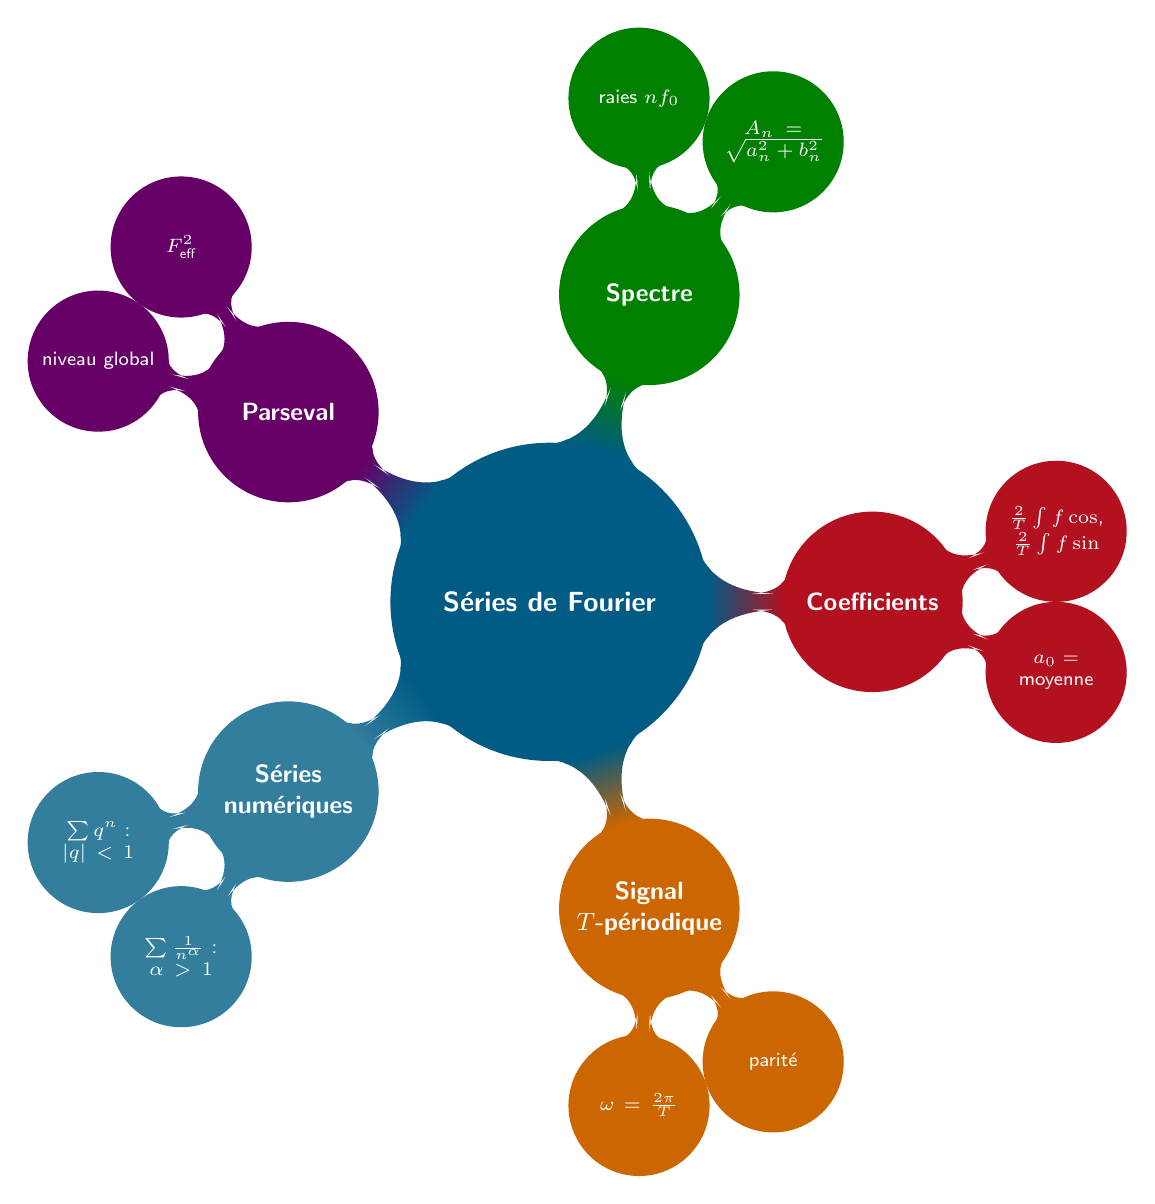
\begin{tikzpicture}[mindmap, grow cyclic, every node/.style={concept, execute at begin node=\hskip0pt},
  concept color=uimmblue, text=white, font=\sffamily\bfseries,
  level 1/.append style={level distance=4.1cm, sibling angle=72, font=\sffamily\small\bfseries},
  level 2/.append style={level distance=2.5cm, sibling angle=42, font=\sffamily\scriptsize}]
\node[font=\sffamily\bfseries] {Séries de Fourier}
  child[concept color=uimmblue!80] { node {Séries numériques}
    child { node {$\sum q^n$ : $|q|<1$} }
    child { node {$\sum\frac{1}{n^\alpha}$ : $\alpha>1$} } }
  child[concept color=orange!80!black] { node {Signal $T$-périodique}
    child { node {$\omega=\frac{2\pi}{T}$} }
    child { node {parité} } }
  child[concept color=uimmred!85!black] { node {Coefficients}
    child { node {$a_0$ = moyenne} }
    child { node {$\frac2T\int f\cos$, $\frac2T\int f\sin$} } }
  child[concept color=green!50!black] { node {Spectre}
    child { node {$A_n=\sqrt{a_n^2+b_n^2}$} }
    child { node {raies $nf_0$} } }
  child[concept color=violet!80!black] { node {Parseval}
    child { node {$F_{\text{eff}}^2$} }
    child { node {niveau global} } };
\end{tikzpicture}
\end{center}

\subsection{Les erreurs fréquentes}\label{subsec:erreurs}

\begin{center}
\renewcommand{\arraystretch}{1.4}
\begin{tabular}{|p{6.8cm}|p{8.6cm}|}
\hline
\rowcolor{uimmlightblue}
\textbf{Erreur} & \textbf{Ce qu'il faut faire} \\
\hline
Utiliser $\frac1T$ devant $a_n$ et $b_n$ & $\frac2T$ pour $a_n$, $b_n$ ; $\frac1T$ pour $a_0$ seulement. \\
\hline
Confondre $\omega$ et $f_0$ & $\omega = 2\pi f_0 = \frac{2\pi}{T}$ (rad/s) ; $f_0 = \frac1T$ (Hz). \\
\hline
Laisser $\cos(n\pi)$ dans le résultat & Remplacer par $(-1)^n$, et $\sin(n\pi)$ par $0$. \\
\hline
Oublier de séparer $n$ pair et $n$ impair & $1-(-1)^n$ vaut $0$ ou $2$ : écrire les deux cas. \\
\hline
Additionner les amplitudes pour la valeur efficace & Additionner les \textbf{carrés} des valeurs efficaces (Parseval). \\
\hline
Oublier $a_0^2$ dans Parseval & Le terme constant compte (sans le facteur $\frac12$). \\
\hline
\end{tabular}
\end{center}

\subsection{Regards croisés : trois professionnels, un même spectre}\label{subsec:regards}

\begin{remarque}[-- Table ronde]
\begin{itemize}
  \item \textbf{L'analyste vibratoire :} « Je ne regarde presque jamais le signal temporel. Sur le spectre, une raie à 1× me parle de balourd, une raie à 2× de désalignement, une raie à $60$× d'engrenage. Fourier me donne la carte d'identité de la machine. »
  \item \textbf{L'électrotechnicien :} « Un onduleur produit un créneau. Ses harmoniques 3, 5, 7 font chauffer le moteur et perturbent le réseau. Je filtre ce que Fourier me montre. »
  \item \textbf{Le technicien qualité :} « Pour qualifier une ligne, je compare le niveau global vibratoire à un seuil. Parseval me dit comment ce niveau se construit à partir des raies, et donc laquelle corriger en priorité. »
\end{itemize}
\end{remarque}

\needspace{12cm}
\subsection{Testez-vous}\label{subsec:quiz}

\begin{exemple}[-- Quiz d'auto-évaluation (réponses en bas de page)]
\begin{enumerate}
  \item La série $\sum_{n\geq0} 0{,}9^n$ converge-t-elle ? Si oui, que vaut sa somme ?
  \item La série $\sum_{n\geq1}\frac{1}{\sqrt n}$ converge-t-elle ?
  \item Un moteur tourne à $3\,000$\,tr/min. Quelle est la fréquence de la raie 2× ?
  \item Un signal est impair. Quels coefficients sont nuls ?
  \item Un signal présente des sauts. Ses amplitudes décroissent-elles en $\frac1n$ ou en $\frac1{n^2}$ ?
  \item Deux raies de vitesse efficace $3$\,mm/s et $4$\,mm/s. Niveau global ?
\end{enumerate}
\vspace{2pt}
\rule{\linewidth}{0.4pt}\\
\footnotesize\textit{Réponses.} 1. Oui, $\frac{1}{1-0{,}9} = 10$. \ 2. Non (Riemann, $\alpha = \frac12\leq 1$). \ 3. $50$\,Hz $\times 2 = 100$\,Hz. \ 4. $a_0$ et tous les $a_n$. \ 5. En $\frac1n$. \ 6. $\sqrt{9+16} = 5$\,mm/s.
\end{exemple}

\subsection{Plan de travail conseillé}\label{subsec:plan}

\begin{center}
\renewcommand{\arraystretch}{1.35}
\begin{tabular}{|c|p{6.5cm}|p{7.5cm}|}
\hline
\rowcolor{uimmlightblue}
\textbf{Étape} & \textbf{Cours} & \textbf{TD (exercices)} \\
\hline
1 & §\ref{sec:series} : séries numériques & Exercices 1 à 3 \\
\hline
2 & §\ref{sec:signaux} : signaux périodiques, parité & Exercices 4 et 5 \\
\hline
3 & §\ref{sec:fourier} : coefficients, spectre & Exercices 6 à 10 \\
\hline
4 & §\ref{sec:convergence} : sommes partielles, identification & Exercices 11 et 12 (GeoGebra) \\
\hline
5 & §\ref{sec:parseval} : Parseval, valeur efficace & Exercices 13 et 14, puis le problème de synthèse \\
\hline
\end{tabular}
\end{center}

\begin{remarque}[-- Pour progresser]
Avant le TP, entraînez-vous à passer dans les deux sens : d'un signal à son spectre (quelles raies ? quelles amplitudes ?) et d'un spectre à l'allure du signal. Notez à chaque exercice le type d'erreur commise ($\omega$ ou $f_0$, facteur $\frac2T$, $n$ pair ou impair) : l'étiquette qui revient désigne le point à retravailler.
\end{remarque}

% ============================================================
\newpage
\section*{Annexe -- Fiches logiciel et calculatrice}\label{sec:annexe}
\addcontentsline{toc}{section}{Annexe -- Fiches logiciel et calculatrice}

\begin{calculatrice}[-- GeoGebra : tracer une somme partielle, calculer un coefficient]\label{fiche:geogebra}
\small
\renewcommand{\arraystretch}{1.35}
\begin{tabular}{@{}>{\bfseries\color{uimmblue}}p{3.3cm}|p{12.6cm}@{}}
Signal créneau ($T = 1$) & \texttt{f(x) = Si(x - floor(x) < 0.5, 1, -1)} \\
\hline
Dent de scie ($T = 1$) & \texttt{g(x) = x - floor(x)} \\
\hline
Curseur pour $N$ & \texttt{N = Curseur(1, 50, 1)} \\
\hline
Somme partielle du créneau & \texttt{S(x) = Somme(4 / (pi (2k - 1)) sin((2k - 1)*2 pi x), k, 1, N)} \quad (harmoniques impairs jusqu'au rang $2N-1$) \\
\hline
Coefficient $b_3$ (valeur approchée) & \texttt{b3 = 2 Intégrale(f(x) sin(2 pi*3 x), 0, 1)} \\
\hline
Coefficient $b_n$ (calcul formel) & Vue \textit{Calcul formel} : \texttt{2 Intégrale(t sin(n*2 pi t), t, 0, 1)}. Le résultat contient $\sin(2n\pi)$ et $\cos(2n\pi)$ : les remplacer par $0$ et $1$. \\
\hline
\end{tabular}

\smallskip
\footnotesize\textit{GeoGebra accepte aussi les noms de commandes anglais (\texttt{If}, \texttt{Sum}, \texttt{Integral}, \texttt{Slider}). Le nombre $\pi$ se saisit \texttt{pi}.}
\end{calculatrice}

\begin{calculatrice}[-- Calculatrices : valeur approchée d'une intégrale]\label{fiche:calc}
\small
\renewcommand{\arraystretch}{1.35}
\begin{tabular}{@{}p{4.9cm}|p{4.9cm}|p{5.6cm}@{}}
\textbf{NumWorks} & \textbf{TI-83 Premium CE} & \textbf{Casio Graph 90+E} \\
\hline
Application \textit{Calculs}, \touche{boîte à outils} $\rightarrow$ \textit{Calcul} $\rightarrow$ \textit{Intégrale}, puis compléter le gabarit $\int_a^b\dots\,\mathrm dx$. &
\touche{math}, puis \texttt{fnInt(} (ou le gabarit d'intégrale) : \texttt{fnInt(expression, X, a, b)}. &
Menu \textit{Exe-Mat}, \touche{OPTN} $\rightarrow$ \textit{CALC} $\rightarrow$ $\int\mathrm dx$, puis compléter le gabarit. \\
\hline
\multicolumn{3}{@{}p{16cm}@{}}{\textbf{Exemple :} $b_1$ du triangle est nul par parité ; pour vérifier $a_1 = \frac{8}{\pi^2}\approx 0{,}8106$ ($E = 1$, $T = 1$), on calcule $4\int_0^{0{,}5}(1-4x)\cos(2\pi x)\,\mathrm dx$ \textbf{en mode radian}.} \\
\end{tabular}

\smallskip
\footnotesize\textit{Les intitulés des menus peuvent varier selon la version du système. Toujours vérifier que la calculatrice est en radians.}
\end{calculatrice}

\end{document}
